\section{Circuitos combinacionais}

\frame{
	\frametitle{Relembrando...}
	
	\centering
	\begin{tikzpicture}[node distance=0.5cm, base/.style={
		% The shape:
		rectangle,minimum height=1cm,minimum width=1.5cm,rounded corners=3mm,align=center,
		% The rest
		very thick,draw=black!50,
		fill=black!20}]
	
	\node[base] (S) {Situação};
	\node[base,right=of S,text width=1.5cm] (TV) {Tabela verdade};
	\node[base, right=of TV, text width=2cm] (ES) {Expressão simplificada};
	\node[base, right=of ES] (C) {Circuito};
	
	\graph {(S) -> (TV) -> (ES) -> (C);};
	
	\end{tikzpicture}
%	\centerline{\includegraphics[width=0.75\linewidth]{Figuras/Ch4/resumo04.png}}
}

\frame{
	\frametitle{Circuitos combinacionais com 2 variáveis - Exemplo \#01}

	\centering
	

\tikzset{every picture/.style={line width=0.75pt}} %set default line width to 0.75pt        

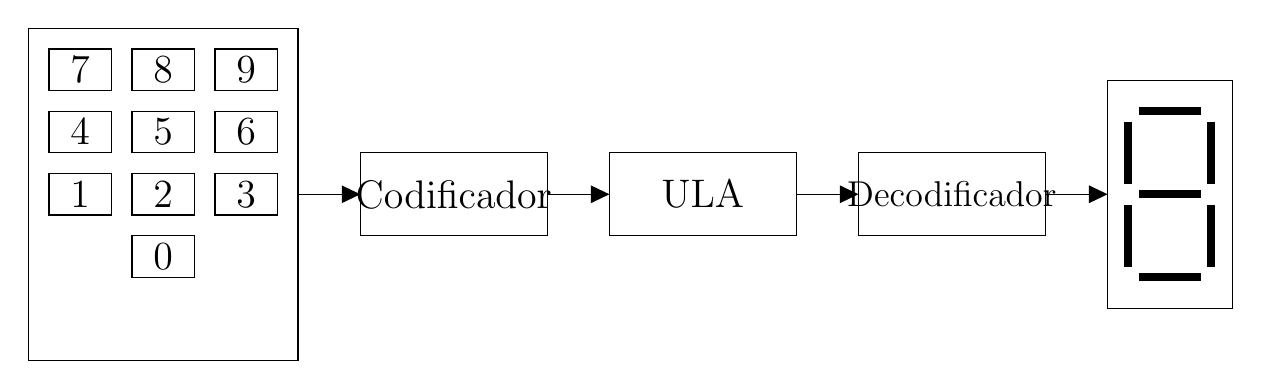
\begin{tikzpicture}[x=0.75pt,y=0.75pt,yscale=-1,xscale=1]
%uncomment if require: \path (0,300); %set diagram left start at 0, and has height of 300

%Shape: Rectangle [id:dp8798188650405219] 
\draw   (30,50) -- (160,50) -- (160,210) -- (30,210) -- cycle ;
%Shape: Rectangle [id:dp593444354888008] 
\draw   (40,60) -- (70,60) -- (70,80) -- (40,80) -- cycle ;
%Shape: Rectangle [id:dp4412846627526852] 
\draw   (80,60) -- (110,60) -- (110,80) -- (80,80) -- cycle ;
%Shape: Rectangle [id:dp2343273962035186] 
\draw   (120,60) -- (150,60) -- (150,80) -- (120,80) -- cycle ;
%Shape: Rectangle [id:dp05777918912875246] 
\draw   (40,90) -- (70,90) -- (70,110) -- (40,110) -- cycle ;
%Shape: Rectangle [id:dp9955010424516375] 
\draw   (80,90) -- (110,90) -- (110,110) -- (80,110) -- cycle ;
%Shape: Rectangle [id:dp24021539717259266] 
\draw   (120,90) -- (150,90) -- (150,110) -- (120,110) -- cycle ;
%Shape: Rectangle [id:dp36169684584711925] 
\draw   (40,120) -- (70,120) -- (70,140) -- (40,140) -- cycle ;
%Shape: Rectangle [id:dp7232437677097003] 
\draw   (80,120) -- (110,120) -- (110,140) -- (80,140) -- cycle ;
%Shape: Rectangle [id:dp6884539525496838] 
\draw   (120,120) -- (150,120) -- (150,140) -- (120,140) -- cycle ;
%Shape: Rectangle [id:dp9961423077173726] 
\draw   (80,150) -- (110,150) -- (110,170) -- (80,170) -- cycle ;
%Shape: Rectangle [id:dp6643057105712631] 
\draw   (190,110) -- (280,110) -- (280,150) -- (190,150) -- cycle ;
%Shape: Rectangle [id:dp7094011053258715] 
\draw   (550,75) -- (610,75) -- (610,185) -- (550,185) -- cycle ;
%Shape: Rectangle [id:dp2693438921699036] 
\draw   (310,110) -- (400,110) -- (400,150) -- (310,150) -- cycle ;
%Shape: Rectangle [id:dp3654960401722005] 
\draw   (430,110) -- (520,110) -- (520,150) -- (430,150) -- cycle ;
%Straight Lines [id:da6667328032348829] 
\draw    (160,130) -- (188,130) ;
\draw [shift={(190,130)}, rotate = 180] [fill={rgb, 255:red, 0; green, 0; blue, 0 }  ][line width=0.75]  [draw opacity=0] (8.93,-4.29) -- (0,0) -- (8.93,4.29) -- cycle    ;

%Straight Lines [id:da5165651690517046] 
\draw    (280,130) -- (308,130) ;
\draw [shift={(310,130)}, rotate = 180] [fill={rgb, 255:red, 0; green, 0; blue, 0 }  ][line width=0.75]  [draw opacity=0] (8.93,-4.29) -- (0,0) -- (8.93,4.29) -- cycle    ;

%Straight Lines [id:da17751850693095572] 
\draw    (400,130) -- (428,130) ;
\draw [shift={(430,130)}, rotate = 180] [fill={rgb, 255:red, 0; green, 0; blue, 0 }  ][line width=0.75]  [draw opacity=0] (8.93,-4.29) -- (0,0) -- (8.93,4.29) -- cycle    ;

%Straight Lines [id:da4998570413390182] 
\draw [color={rgb, 255:red, 0; green, 0; blue, 0 }  ,draw opacity=1 ][line width=3]    (560,95) -- (560,125) ;


%Straight Lines [id:da05287212083080073] 
\draw [color={rgb, 255:red, 0; green, 0; blue, 0 }  ,draw opacity=1 ][line width=3]    (600,95) -- (600,125) ;


%Straight Lines [id:da9146969001147236] 
\draw [color={rgb, 255:red, 0; green, 0; blue, 0 }  ,draw opacity=1 ][line width=3]    (560,135) -- (560,165) ;


%Straight Lines [id:da37610179690179124] 
\draw [color={rgb, 255:red, 0; green, 0; blue, 0 }  ,draw opacity=1 ][line width=3]    (600,135) -- (600,165) ;


%Straight Lines [id:da2798262228013664] 
\draw [color={rgb, 255:red, 0; green, 0; blue, 0 }  ,draw opacity=1 ][line width=3]    (595,130) -- (565,130) ;


%Straight Lines [id:da15184615547446478] 
\draw [color={rgb, 255:red, 0; green, 0; blue, 0 }  ,draw opacity=1 ][line width=3]    (595,90) -- (565,90) ;


%Straight Lines [id:da20609816632014244] 
\draw [color={rgb, 255:red, 0; green, 0; blue, 0 }  ,draw opacity=1 ][line width=3]    (595,170) -- (565,170) ;


%Straight Lines [id:da16937059284664002] 
\draw    (520,130) -- (548,130) ;
\draw [shift={(550,130)}, rotate = 180] [fill={rgb, 255:red, 0; green, 0; blue, 0 }  ][line width=0.75]  [draw opacity=0] (8.93,-4.29) -- (0,0) -- (8.93,4.29) -- cycle    ;


% Text Node
\draw (135,70) node   {\Large $9$};
% Text Node
\draw (95,70) node   {\Large $8$};
% Text Node
\draw (55,70) node   {\Large $7$};
% Text Node
\draw (135,100) node   {\Large $6$};
% Text Node
\draw (135,130) node   {\Large $3$};
% Text Node
\draw (95,160) node   {\Large $0$};
% Text Node
\draw (95,130) node   {\Large $2$};
% Text Node
\draw (95,100) node   {\Large $5$};
% Text Node
\draw (55,100) node   {\Large $4$};
% Text Node
\draw (55,130) node   {\Large $1$};
% Text Node
\draw (235,130) node  [align=left] {\Large Codificador};
% Text Node
\draw (355,130) node  [align=left] {\Large ULA};
% Text Node
\draw (475,130) node [scale=0.9] [align=left] {\Large Decodificador};


\end{tikzpicture}

%	\centerline{\includegraphics[width=0.75\linewidth]{Figuras/Ch4/2var.PNG}}
}

\frame{
	\frametitle{Circuitos combinacionais com 2 variáveis - Exemplo \#01}
	\begin{block}{}
		Deseja-se instalar, no cruzamento, um sistema automático de semáforos, com as seguintes características:
		\begin{itemize}
			\item Quando houver carros transitando somente na rua B, o semáforo 2 deverá permanecer verde para os carros trafegarem livremente.
			\item Igualmente, quando houver carros transitando somente na rua A, o semáforo 1 deverá permanecer verde.
			\item Quando houver carros transitando em ambas as ruas, o semáforo da rua A deve ficar verde, pois é a rua preferencial.
		\end{itemize}
	\end{block}

}


\frame{
	\frametitle{Circuitos combinacionais com 2 variáveis - Exemplo \#01}
		\centering
		\begin{tabular}{cc|cccc}
			\toprule
			A & B & G1 & R1 & G2 & R2 \\ \midrule
			0 & 0 &    &    &    &    \\
			0 & 1 &    &    &    &    \\
			1 & 0 &    &    &    &    \\
			1 & 1 &    &    &    &    \\ \bottomrule
		\end{tabular}
}

\frame{
	\frametitle{Circuitos combinacionais com 2 variáveis - Exemplo \#01}
		\centering
		\begin{tabular}{cc|cccc}
			\toprule
			A                & B                & G1 & R1 & G2 & R2 \\ \midrule
			\textcolor{red}0 & \textcolor{red}0 &    &    &    &    \\
			0                & 1                &    &    &    &    \\
			1                & 0                &    &    &    &    \\
			1                & 1                &    &    &    &    \\ \bottomrule
		\end{tabular}
}

\frame{
	\frametitle{Circuitos combinacionais com 2 variáveis - Exemplo \#01}
		\centering
		\begin{tabular}{cc|cccc}
			\toprule
			A                & B                & G1                 & R1                 & G2                 & R2                 \\ \midrule
			\textcolor{red}0 & \textcolor{red}0 & \textcolor{blue} X & \textcolor{blue} X & \textcolor{blue} X & \textcolor{blue} X \\
			0                & 1                &                    &                    &                    &                    \\
			1                & 0                &                    &                    &                    &                    \\
			1                & 1                &                    &                    &                    &                    \\ \bottomrule
		\end{tabular}
}

\frame{
	\frametitle{Circuitos combinacionais com 2 variáveis - Exemplo \#01}
		\centering
		\begin{tabular}{cc|cccc}
			\toprule
			A                & B                & G1 & R1 & G2 & R2 \\ \midrule
			0                & 0                & X  & X  & X  & X  \\ 
			\textcolor{red}0 & \textcolor{red}1 &    &    &    &    \\ 
			1                & 0                &    &    &    &    \\ 
			1                & 1                &    &    &    &    \\ \bottomrule
		\end{tabular}
}

\frame{
	\frametitle{Circuitos combinacionais com 2 variáveis - Exemplo \#01}
		\centering
		\begin{tabular}{cc|cccc}
			\toprule
			A                & B                & G1                & R1                & G2                & R2                \\ \midrule
			0                & 0                & X                 & X                 & X                 & X                 \\ 
			\textcolor{red}0 & \textcolor{red}1 & \textcolor{blue}0 & \textcolor{blue}1 & \textcolor{blue}1 & \textcolor{blue}0 \\ 
			1                & 0                &                   &                   &                   &                   \\ 
			1                & 1                &                   &                   &                   &                   \\ \bottomrule
		\end{tabular}
}

\frame{
	\frametitle{Circuitos combinacionais com 2 variáveis - Exemplo \#01}
		\centering
		\begin{tabular}{cc|cccc}
			\toprule
			A                & B                & G1 & R1 & G2 & R2 \\ \midrule
			0                & 0                & X  & X  & X  & X  \\ 
			0                & 1                & 0  & 1  & 1  & 0  \\ 
			\textcolor{red}1 & \textcolor{red}0 &    &    &    &    \\ 
			1                & 1                &    &    &    &    \\ \bottomrule
		\end{tabular}
}

\frame{
	\frametitle{Circuitos combinacionais com 2 variáveis - Exemplo \#01}
		\centering
		\begin{tabular}{cc|cccc}
			\toprule
			A                & B                & G1                & R1                & G2                & R2                \\ \midrule
			0                & 0                & X                 & X                 & X                 & X                 \\ 
			0                & 1                & 0                 & 1                 & 1                 & 0                 \\ 
			\textcolor{red}1 & \textcolor{red}0 & \textcolor{blue}1 & \textcolor{blue}0 & \textcolor{blue}0 & \textcolor{blue}1 \\ 
			1                & 1                &                   &                   &                   &                   \\ \bottomrule
		\end{tabular}
}

\frame{
	\frametitle{Circuitos combinacionais com 2 variáveis - Exemplo \#01}
		\centering
		\begin{tabular}{cc|cccc}
			\toprule
			A                & B                & G1 & R1 & G2 & R2 \\ \midrule
			0                & 0                & X  & X  & X  & X  \\ 
			0                & 1                & 0  & 1  & 1  & 0  \\ 
			1                & 0                & 1  & 0  & 0  & 1  \\ 
			\textcolor{red}1 & \textcolor{red}1 &    &    &    &    \\ \bottomrule
		\end{tabular}
}

\frame{
	\frametitle{Circuitos combinacionais com 2 variáveis - Exemplo \#01}
		\centering
		\begin{tabular}{cc|cccc}
			\toprule
			A                & B                & G1                & R1                & G2                & R2                \\ \midrule
			0                & 0                & X                 & X                 & X                 & X                 \\ 
			0                & 1                & 0                 & 1                 & 1                 & 0                 \\ 
			1                & 0                & 1                 & 0                 & 0                 & 1                 \\ 
			\textcolor{red}1 & \textcolor{red}1 & \textcolor{blue}1 & \textcolor{blue}0 & \textcolor{blue}0 & \textcolor{blue}1 \\ \bottomrule
		\end{tabular}
}

\frame{
	\frametitle{Circuitos combinacionais com 2 variáveis - Exemplo \#01}
		\centering
		\begin{tabular}{cc|cccc}
			\toprule
			A & B & G1 & R1 & G2 & R2            \\ \midrule
			0 & 0 & X  & X  & X  & X             \\ 
			0 & 1 & 0  & 1  & 1  & 0             \\ 
			1 & 0 & 1  & 0  & 0  & 1             \\ 
			1 & 1 & 1  & 0  & 0  & 1             \\ \bottomrule
		\end{tabular}
}

\frame{
\frametitle{Circuitos combinacionais com 2 variáveis - Exemplo \#01}

\begin{center}

\begin{karnaugh-map}[2][2][1][$A$][$B$]
\manualterms{X,1,0,1}
\implicant{1}{3}
\end{karnaugh-map}

\begin{block}{Expressão simplificada}
	\[ G1 = {\color{red} A} \]
\end{block}

\end{center}
}

\frame{
\frametitle{Circuitos combinacionais com 2 variáveis - Exemplo \#01}

\begin{center}

\begin{karnaugh-map}[2][2][1][$A$][$B$]
\manualterms{X,0,1,0}
\implicant{0}{2}
\end{karnaugh-map}

\begin{block}{Expressão simplificada}
	\[ R1 = {\color{red} \notted{A}} \]
\end{block}

\end{center}
}

\frame{
\frametitle{Circuitos combinacionais com 2 variáveis - Exemplo \#01}

\begin{center}

\begin{karnaugh-map}[2][2][1][$A$][$B$]
\manualterms{X,0,1,0}
\implicant{0}{2}
\end{karnaugh-map}

\begin{block}{Expressão simplificada}
	\[ G2 = {\color{red} \notted{A}} \]
\end{block}

\end{center}
}

\frame{
\frametitle{Circuitos combinacionais com 2 variáveis - Exemplo \#01}

\begin{center}

\begin{karnaugh-map}[2][2][1][$A$][$B$]
\manualterms{X,1,0,1}
\implicant{1}{3}
\end{karnaugh-map}

\begin{block}{Expressão simplificada}
	\[ R2 = {\color{red} A} \]
\end{block}

\end{center}
}

\frame{
	\frametitle{Circuitos combinacionais com 3 variáveis - Exemplo \#02}
	\centerline{\includegraphics[width=1\linewidth]{Figuras/Ch4/3var.PNG}}
}

\frame{
	\frametitle{Circuitos combinacionais com 3 variáveis - Exemplo \#02}

	\begin{block}{}
		Deseja-se instalar um amplificador para ligar três aparelhos, com as seguintes prioridades: 
		
		\begin{itemize}
			\item Prioridade 1: CD player
			\item Prioridade 2: Tape playback
			\item Prioridade 3: Rádio receptor
		\end{itemize}
	\end{block}
}

\frame{
	\frametitle{Circuitos combinacionais com 3 variáveis - Exemplo \#02}
		\centering
		\begin{tabular}{ccc|ccc}
			\toprule
			A & B & C & SA & SB & SC             \\ \midrule
			0 & 0 & 0 &    &    &                \\ 
			0 & 0 & 1 &    &    &                \\ 
			0 & 1 & 0 &    &    &                \\ 
			0 & 1 & 1 &    &    &                \\ 
			1 & 0 & 0 &    &    &                \\ 
			1 & 0 & 1 &    &    &                \\ 
			1 & 1 & 0 &    &    &                \\ 
			1 & 1 & 1 &    &    &                \\ \bottomrule
		\end{tabular}
}

\frame{
	\frametitle{Circuitos combinacionais com 3 variáveis - Exemplo \#02}
		\centering
		\begin{tabular}{ccc|ccc}
			\toprule
			A                & B & C & SA & SB & SC \\ \midrule
			\textcolor{red}0 &
			\textcolor{red}0 &
			\textcolor{red}0 &   &   &              \\ 
			0                & 0 & 1 &    &    &    \\ 
			0                & 1 & 0 &    &    &    \\ 
			0                & 1 & 1 &    &    &    \\ 
			1                & 0 & 0 &    &    &    \\ 
			1                & 0 & 1 &    &    &    \\ 
			1                & 1 & 0 &    &    &    \\ 
			1                & 1 & 1 &    &    &    \\ \bottomrule
		\end{tabular}
}

\frame{
	\frametitle{Circuitos combinacionais com 3 variáveis - Exemplo \#02}
		\centering
		\begin{tabular}{ccc|ccc}
			\toprule
			A                & B                 & C                 & SA                & SB & SC \\ \midrule
			\textcolor{red}0 &
			\textcolor{red}0 &
			\textcolor{red}0 & \textcolor{blue}X & \textcolor{blue}X & \textcolor{blue}X           \\ 
			0                & 0                 & 1                 &                   &    &    \\ 
			0                & 1                 & 0                 &                   &    &    \\ 
			0                & 1                 & 1                 &                   &    &    \\ 
			1                & 0                 & 0                 &                   &    &    \\ 
			1                & 0                 & 1                 &                   &    &    \\ 
			1                & 1                 & 0                 &                   &    &    \\ 
			1                & 1                 & 1                 &                   &    &    \\ \bottomrule
		\end{tabular}
}


\frame{
	\frametitle{Circuitos combinacionais com 3 variáveis - Exemplo \#02}
		\centering
		\begin{tabular}{ccc|ccc}\toprule
			A                & B                & C                & SA & SB & SC \\ \midrule
			0                & 0                & 0                & X  & X  & X  \\ 
			\textcolor{red}0 & \textcolor{red}0 & \textcolor{red}1 &    &    &    \\ 
			0                & 1                & 0                &    &    &    \\ 
			0                & 1                & 1                &    &    &    \\ 
			1                & 0                & 0                &    &    &    \\ 
			1                & 0                & 1                &    &    &    \\ 
			1                & 1                & 0                &    &    &    \\ 
			1                & 1                & 1                &    &    &    \\ \bottomrule
		\end{tabular}
}

\frame{
	\frametitle{Circuitos combinacionais com 3 variáveis - Exemplo \#02}
		\centering
		\begin{tabular}{ccc|ccc}
			\toprule
			A                & B                & C                & SA                & SB                & SC                \\ \midrule
			0                & 0                & 0                & X                 & X                 & X                 \\ 
			\textcolor{red}0 & \textcolor{red}0 & \textcolor{red}1 & \textcolor{blue}0 & \textcolor{blue}0 & \textcolor{blue}1 \\ 
			0                & 1                & 0                &                   &                   &                   \\ 
			0                & 1                & 1                &                   &                   &                   \\ 
			1                & 0                & 0                &                   &                   &                   \\ 
			1                & 0                & 1                &                   &                   &                   \\ 
			1                & 1                & 0                &                   &                   &                   \\ 
			1                & 1                & 1                &                   &                   &                   \\ \bottomrule
		\end{tabular}
}

\frame{
	\frametitle{Circuitos combinacionais com 3 variáveis - Exemplo \#02}
		\centering
		\begin{tabular}{ccc|ccc}
			\toprule
			A                & B                & C                & SA & SB & SC \\ \midrule
			0                & 0                & 0                & X  & X  & X  \\ 
			0                & 0                & 1                & 0  & 0  & 1  \\ 
			\textcolor{red}0 & \textcolor{red}1 & \textcolor{red}0 &    &    &    \\ 
			0                & 1                & 1                &    &    &    \\ 
			1                & 0                & 0                &    &    &    \\ 
			1                & 0                & 1                &    &    &    \\ 
			1                & 1                & 0                &    &    &    \\ 
			1                & 1                & 1                &    &    &    \\ \bottomrule
		\end{tabular}
}

\frame{
	\frametitle{Circuitos combinacionais com 3 variáveis - Exemplo \#02}
		\centering
		\begin{tabular}{ccc|ccc}
			\toprule
			A                & B                & C                & SA                & SB                & SC                \\ \midrule
			0                & 0                & 0                & X                 & X                 & X                 \\ 
			0                & 0                & 1                & 0                 & 0                 & 1                 \\ 
			\textcolor{red}0 & \textcolor{red}1 & \textcolor{red}0 & \textcolor{blue}0 & \textcolor{blue}1 & \textcolor{blue}0 \\ 
			0                & 1                & 1                &                   &                   &                   \\ 
			1                & 0                & 0                &                   &                   &                   \\ 
			1                & 0                & 1                &                   &                   &                   \\ 
			1                & 1                & 0                &                   &                   &                   \\ 
			1                & 1                & 1                &                   &                   &                   \\ \bottomrule
		\end{tabular}
}

\frame{
	\frametitle{Circuitos combinacionais com 3 variáveis - Exemplo \#02}
		\centering
		\begin{tabular}{ccc|ccc}
			\toprule
			A                & B                & C                & SA & SB & SC \\ \midrule
			0                & 0                & 0                & X  & X  & X  \\ 
			0                & 0                & 1                & 0  & 0  & 1  \\ 
			0                & 1                & 0                & 0  & 1  & 0  \\ 
			\textcolor{red}0 & \textcolor{red}1 & \textcolor{red}1 &    &    &    \\ 
			1                & 0                & 0                &    &    &    \\ 
			1                & 0                & 1                &    &    &    \\ 
			1                & 1                & 0                &    &    &    \\ 
			1                & 1                & 1                &    &    &    \\ \bottomrule
		\end{tabular}
}

\frame{
	\frametitle{Circuitos combinacionais com 3 variáveis - Exemplo \#02}
		\centering
		\begin{tabular}{ccc|ccc}
			\toprule
			A                & B                & C                & SA                & SB                & SC                \\ \midrule
			0                & 0                & 0                & X                 & X                 & X                 \\ 
			0                & 0                & 1                & 0                 & 0                 & 1                 \\ 
			0                & 1                & 0                & 0                 & 1                 & 0                 \\ 
			\textcolor{red}0 & \textcolor{red}1 & \textcolor{red}1 & \textcolor{blue}0 & \textcolor{blue}1 & \textcolor{blue}0 \\ 
			1                & 0                & 0                &                   &                   &                   \\ 
			1                & 0                & 1                &                   &                   &                   \\ 
			1                & 1                & 0                &                   &                   &                   \\ 
			1                & 1                & 1                &                   &                   &                   \\ \bottomrule
		\end{tabular}
}


\frame{
	\frametitle{Circuitos combinacionais com 3 variáveis - Exemplo \#02}
		\centering
		\begin{tabular}{ccc|ccc}
			\toprule
			A                & B                & C                & SA & SB & SC \\ \midrule
			0                & 0                & 0                & X  & X  & X  \\ 
			0                & 0                & 1                & 0  & 0  & 1  \\ 
			0                & 1                & 0                & 0  & 1  & 0  \\ 
			0                & 1                & 1                & 0  & 1  & 0  \\ 
			\textcolor{red}1 & \textcolor{red}0 & \textcolor{red}0 &    &    &    \\ 
			1                & 0                & 1                &    &    &    \\ 
			1                & 1                & 0                &    &    &    \\ 
			1                & 1                & 1                &    &    &    \\ \bottomrule
		\end{tabular}
}

\frame{
	\frametitle{Circuitos combinacionais com 3 variáveis - Exemplo \#02}
		\centering
		\begin{tabular}{ccc|ccc}
			\toprule
			A                & B                & C                & SA                & SB                & SC                \\ \midrule
			0                & 0                & 0                & X                 & X                 & X                 \\ 
			0                & 0                & 1                & 0                 & 0                 & 1                 \\ 
			0                & 1                & 0                & 0                 & 1                 & 0                 \\ 
			0                & 1                & 1                & 0                 & 1                 & 0                 \\ 
			\textcolor{red}1 & \textcolor{red}0 & \textcolor{red}0 & \textcolor{blue}1 & \textcolor{blue}0 & \textcolor{blue}0 \\ 
			1                & 0                & 1                &                   &                   &                   \\ 
			1                & 1                & 0                &                   &                   &                   \\ 
			1                & 1                & 1                &                   &                   &                   \\ \bottomrule
		\end{tabular}
}

\frame{
	\frametitle{Circuitos combinacionais com 3 variáveis - Exemplo \#02}
		\centering
		\begin{tabular}{ccc|ccc}
			\toprule
			A                & B                & C                & SA & SB & SC \\ \midrule
			0                & 0                & 0                & X  & X  & X  \\ 
			0                & 0                & 1                & 0  & 0  & 1  \\ 
			0                & 1                & 0                & 0  & 1  & 0  \\ 
			0                & 1                & 1                & 0  & 1  & 0  \\ 
			1                & 0                & 0                & 1  & 0  & 0  \\ 
			\textcolor{red}1 & \textcolor{red}0 & \textcolor{red}1 &    &    &    \\ 
			1                & 1                & 0                &    &    &    \\ 
			1                & 1                & 1                &    &    &    \\ \bottomrule
		\end{tabular}
}

\frame{
	\frametitle{Circuitos combinacionais com 3 variáveis - Exemplo \#02}
		\centering
		\begin{tabular}{ccc|ccc}
			\toprule
			A                & B                & C                & SA                & SB                & SC                \\ \midrule
			0                & 0                & 0                & X                 & X                 & X                 \\ 
			0                & 0                & 1                & 0                 & 0                 & 1                 \\ 
			0                & 1                & 0                & 0                 & 1                 & 0                 \\ 
			0                & 1                & 1                & 0                 & 1                 & 0                 \\ 
			1                & 0                & 0                & 1                 & 0                 & 0                 \\ 
			\textcolor{red}1 & \textcolor{red}0 & \textcolor{red}1 & \textcolor{blue}1 & \textcolor{blue}0 & \textcolor{blue}0 \\ 
			1                & 1                & 0                &                   &                   &                   \\ 
			1                & 1                & 1                &                   &                   &                   \\ \bottomrule
		\end{tabular}
}

\frame{
	\frametitle{Circuitos combinacionais com 3 variáveis - Exemplo \#02}
		\centering
		\begin{tabular}{ccc|ccc}
			\toprule
			A                & B                & C                & SA & SB & SC \\ \midrule
			0                & 0                & 0                & X  & X  & X  \\ 
			0                & 0                & 1                & 0  & 0  & 1  \\ 
			0                & 1                & 0                & 0  & 1  & 0  \\ 
			0                & 1                & 1                & 0  & 1  & 0  \\ 
			1                & 0                & 0                & 1  & 0  & 0  \\ 
			1                & 0                & 1                & 1  & 0  & 0  \\ 
			\textcolor{red}1 & \textcolor{red}1 & \textcolor{red}0 &    &    &    \\ 
			1                & 1                & 1                &    &    &    \\ \bottomrule
		\end{tabular}
}

\frame{
	\frametitle{Circuitos combinacionais com 3 variáveis - Exemplo \#02}
		\centering
		\begin{tabular}{ccc|ccc}
			\toprule
			A                & B                & C                & SA                & SB                & SC                \\ \midrule
			0                & 0                & 0                & X                 & X                 & X                 \\ 
			0                & 0                & 1                & 0                 & 0                 & 1                 \\ 
			0                & 1                & 0                & 0                 & 1                 & 0                 \\ 
			0                & 1                & 1                & 0                 & 1                 & 0                 \\ 
			1                & 0                & 0                & 1                 & 0                 & 0                 \\ 
			1                & 0                & 1                & 1                 & 0                 & 0                 \\ 
			\textcolor{red}1 & \textcolor{red}1 & \textcolor{red}0 & \textcolor{blue}1 & \textcolor{blue}0 & \textcolor{blue}0 \\ 
			1                & 1                & 1                &                   &                   &                   \\ \bottomrule
		\end{tabular}
}

\frame{
	\frametitle{Circuitos combinacionais com 3 variáveis - Exemplo \#02}
		\centering
		\begin{tabular}{ccc|ccc}
			\toprule
			A                & B                & C                & SA & SB & SC \\ \midrule
			0                & 0                & 0                & X  & X  & X  \\ 
			0                & 0                & 1                & 0  & 0  & 1  \\ 
			0                & 1                & 0                & 0  & 1  & 0  \\ 
			0                & 1                & 1                & 0  & 1  & 0  \\ 
			1                & 0                & 0                & 1  & 0  & 0  \\ 
			1                & 0                & 1                & 1  & 0  & 0  \\ 
			1                & 1                & 0                & 1  & 0  & 0  \\ 
			\textcolor{red}1 & \textcolor{red}1 & \textcolor{red}1 &    &    &    \\ \bottomrule
		\end{tabular}
}

\frame{
	\frametitle{Circuitos combinacionais com 3 variáveis - Exemplo \#02}
		\centering
		\begin{tabular}{ccc|ccc}
			\toprule
			A                & B                & C                & SA                & SB                & SC                \\ \midrule
			0                & 0                & 0                & X                 & X                 & X                 \\ 
			0                & 0                & 1                & 0                 & 0                 & 1                 \\ 
			0                & 1                & 0                & 0                 & 1                 & 0                 \\ 
			0                & 1                & 1                & 0                 & 1                 & 0                 \\ 
			1                & 0                & 0                & 1                 & 0                 & 0                 \\ 
			1                & 0                & 1                & 1                 & 0                 & 0                 \\ 
			1                & 1                & 0                & 1                 & 0                 & 0                 \\ 
			\textcolor{red}1 & \textcolor{red}1 & \textcolor{red}1 & \textcolor{blue}1 & \textcolor{blue}0 & \textcolor{blue}0 \\ \bottomrule
		\end{tabular}
}

\frame{
	\frametitle{Circuitos combinacionais com 3 variáveis - Exemplo \#02}
		\centering
		\begin{tabular}{ccc|ccc}
			\toprule
			A & B & C & SA & SB & SC             \\ \midrule
			0 & 0 & 0 & X  & X  & X              \\ 
			0 & 0 & 1 & 0  & 0  & 1              \\ 
			0 & 1 & 0 & 0  & 1  & 0              \\ 
			0 & 1 & 1 & 0  & 1  & 0              \\ 
			1 & 0 & 0 & 1  & 0  & 0              \\ 
			1 & 0 & 1 & 1  & 0  & 0              \\ 
			1 & 1 & 0 & 1  & 0  & 0              \\ 
			1 & 1 & 1 & 1  & 0  & 0              \\ \bottomrule
		\end{tabular}
}

\frame{
\frametitle{Circuitos combinacionais com 3 variáveis - Exemplo \#02}

\begin{center}

\begin{karnaugh-map}[4][2][1][$AB$][$C$]
\manualterms{X,0,1,1,0,0,1,1}
\implicant{3}{6}
\end{karnaugh-map}

\begin{block}{Expressão simplificada}
	\[ SA = {\color{red} A} \]
\end{block}

\end{center}
}

\frame{
\frametitle{Circuitos combinacionais com 3 variáveis - Exemplo \#02}

\begin{center}

\begin{karnaugh-map}[4][2][1][$AB$][$C$]
\manualterms{X,1,0,0,0,1,0,0}
\implicant{1}{5}
\end{karnaugh-map}

\begin{block}{Expressão simplificada}
	\[ SB = {\color{red} \notted{A}\cdot B} \]
\end{block}

\end{center}
}

\frame{
\frametitle{Circuitos combinacionais com 3 variáveis - Exemplo \#02}

\begin{center}

\begin{karnaugh-map}[4][2][1][$AB$][$C$]
\manualterms{X,0,0,0,1,0,0,0}
\implicant{0}{4}
\end{karnaugh-map}

\begin{block}{Expressão simplificada}
	\[ SC = {\color{red} \notted{A}\cdot \notted{B}} \]
\end{block}

\end{center}
}


\section*{Exercícios}

\frame{
	\frametitle{Exercícios}
	\begin{block}{}
		01. Quatro juízes participam de um programa de calouros e cada um tem a sua disposição, uma chave liga/desliga correspondendo ao julgamento do candidato: aprovado ou reprovado. Na saída existem três lâmpadas, correspondentes a três resultados: aprovado (pela maioria), reprovado (pela maioria) ou empate.
		
		\bigskip
		
		02. Um motor deve funcionar quando uma ou mais das seguintes condições forem satisfeitas: \textbf{(1)} Regime de carga $\geqslant 80\%$ e Temperatura $> \SI{25}{\degreeCelsius}$; \textbf{(2)} Regime de carga $< 80\%$, Umidade relativa $>60\%$ e Temperatura $> \SI{25}{\degreeCelsius}$; \textbf{(3)} Regime de carga $< 80\%$, no período de carga entre as \SI{15}{\hour} e \SI{16}{\hour}; \textbf{(4)} Temperatura $> \SI{25}{\degreeCelsius}$, fora do período de carga entre as \SI{15}{\hour} e \SI{16}{\hour}.
		
		\bigskip
		
		03. Projete um circuito digital com 4 variáveis de entrada, que indique quando há um número primo	presente na entrada.
	\end{block}
}


\section*{Referências}


\frame{
	\frametitle{Referências e exercícios complementares}
	\begin{itemize}
		\item IDOETA, Ivan V. e CAPUANO, Francisco G. Elementos de Eletrônica Digital. São Paulo:
		      Editora Érica, ed. 40. 2008.
	\end{itemize}

	\centering{\alert{Página 174 - \textbf{4.3.1 até 4.3.8}}}

}